\documentclass[9pt,spanish,aspectratio=1610]{beamer}
\usepackage[utf8]{inputenc}
\usepackage{amsmath}
\usepackage{graphicx}
\usepackage{amssymb}
\usepackage[spanish]{babel}
\spanishdecimal{.}
\usepackage{subfig}
\usepackage{fancyhdr}
\usepackage{pstricks}
\usepackage[ruled]{algorithm2e}
%\usepackage{ragged2e}
%\usepackage[natbibapa]{apacite}
% \bibliographystyle{apacite} % This is the style you should use with `apacite`.
%\justifying
\DeclareMathOperator{\atantwo}{atan2}
\newcommand\ddfrac[2]{\frac{\displaystyle #1}{\displaystyle #2}}
\usetheme{Boadilla}
\setbeamercovered{transparent}
\beamertemplatenavigationsymbolsempty
\setbeamertemplate{frametitle}
{
  \leavevmode
  \hbox{
  \begin{beamercolorbox}[wd=0.6\paperwidth,left]{frametitle}
    \usebeamerfont{frametitle}\insertframetitle
  \end{beamercolorbox}
  \begin{beamercolorbox}[wd=0.4\paperwidth,center]{frametitle}
    \usebeamerfont{frametitle}\hfill%\small{\thesection. \insertsection}
  \end{beamercolorbox}
  }
}
\setbeamertemplate{footline}
{
  \leavevmode%
  \hbox{%
    \begin{beamercolorbox}[colsep=-0.5pt,wd=.33\paperwidth,ht=3ex,dp=1.5ex,center]{author in head/foot}%
      \usebeamerfont{author in head/foot}\insertshortauthor~~ (\insertshortinstitute)
    \end{beamercolorbox}%
    \begin{beamercolorbox}[colsep=-0.5pt,wd=.34\paperwidth,ht=3ex,dp=1.5ex,center]{date in head/foot}%
      \usebeamerfont{author in head/foot}\insertshorttitle
    \end{beamercolorbox}%
    \begin{beamercolorbox}[colsep=-0.5pt,wd=.33\paperwidth,ht=3ex,dp=1.5ex,right]{author in head/foot}%
      \usebeamerfont{author in head/foot}\insertshortdate{}\hspace*{2em}\scriptsize{\insertframenumber{}}\hspace*{1ex}
    \end{beamercolorbox}
  }
}

\begin{document}
\renewcommand{\tablename}{Tabla}
\renewcommand{\figurename}{Figura}

\title[Object Recognition using Fault Reconstruction Techniques]{Object Recognition by Physical Properties Detection using Fault Reconstruction Techniques}
\author[Marco Negrete and Jesús Savage]{Marco Negrete and Jesús Savage}
\date[RFC-MathWorks Support for Research Projects 2020]{Proposal for the RCF and MathWorks Support for Research Projects 2020}
\institute[FI, UNAM]{Faculty of Engineering, UNAM}

\begin{frame}
\titlepage
\end{frame}

\begin{frame}\frametitle{Objectives and Goals}
  \textbf{Objectives:}
  \begin{itemize}
  \item Applying model based fault signal reconstruction algorithms (MBFRA) to improve manipulation tasks in domestic service robots.
  \item Use an sliding mode observer to estimate the weight of the object being manipulated by the robot.
  \item Implement the developments in ROS nodes.
  \end{itemize}

  \textbf{Goals:}
  \begin{itemize}
  \item Obtain a model of the manipulator from current URDF (using Simscape or Robotics Toolbox) (\textbf{check})
  \item Implement a system identication algorithm 
  \item Design a sliding mode observer to estimate the joint velocities (\textbf{check})
  \item Use the output injection term to estimate the weight being carried by the robot (\textbf{check})
  \item Export estimators from Matlab to ROS nodes (\textbf{check})
  \end{itemize}
\end{frame}

\begin{frame}\frametitle{Simscape model}
  \begin{itemize}
  \item Model was obtained from the original version of Justina's urdf (see left figure). 
  \item Contrary to the last report, at this stage we are using the full 7-DOF manipulator. 
  \end{itemize}
  \begin{columns}
    \begin{column}{0.5\textwidth}
      \begin{figure}
        \centering
        \includegraphics[width=0.3\textwidth]{Figures/justina_urdf.png}
      \end{figure}
    \end{column}
    \begin{column}{0.5\textwidth}
      \begin{figure}
        \centering
        \includegraphics[width=0.4\textwidth]{Figures/left_arm.png}
      \end{figure}
    \end{column}
  \end{columns}
\end{frame}

\begin{frame}\frametitle{Dynamic model}
  Sliding Mode Observers (SMO) were proposed as the method to estimate the mass of the manipulated object. Thus, we need first to obtain the dynamic model.\\
  From the Langrangian of the manipulator, a dynamic model of the following form can be obtained:
  \begin{equation}
    M(q)\ddot{q} + C(q, \dot{q})\dot{q} + B\dot{q} + G(q) + \Delta(q,\dot{q}, u) = u
    \label{eq:lagrangian}
  \end{equation}
  where $q\in \mathbb{R}^7$ are the joint angles, $M(q)\in \mathbb{R}^{7\times 7}$ is the inertia matrix, $C(q,\dot{q})\in \mathbb{R}^{7\times 7}$ is the Matrix of Coriollis forces, $B\dot{q}\in \mathbb{R}^7$ is the vector of friction forces, $G(q)\in\mathbb{R}^7$ is the vector of gravitational forces, $u$ is the input torque, considered as control signal, and $\Delta(q,\dot{q},u)$ is a vector containing all errors due to uncertanties and disturbances. \\
  To design a SMO is necessary to write the model in variable states form. Let $x_1 = [q_1\;q_2\;q_3\;q_4\;q_5\;q_6\;q_7]^T$ and $x_2 = [\dot{q}_1\;\dot{q}_2\;\dot{q}_3\;\dot{q}_4\;\dot{q}_5\;\dot{q}_6\;\dot{q}_7]^T$ be the state variables. Then (\ref{eq:lagrangian}) can be written as:
  \begin{eqnarray}
    \dot{x}_1 &=& x_2\label{eq:model1}\\
    \dot{x}_2 &=& -M^{-1}(q)\left(C(q, \dot{q})\dot{q} + B\dot{q} + G(q) + \Delta(q,\dot{q},u) - u\right)\label{eq:model2}
  \end{eqnarray}
Equation (\ref{eq:model2} ) can also be written in the form:
  \begin{equation*}
    \dot{x}_2 = f(x_1, x_2, u) + g(x_1, x_2, u)
  \end{equation*}
  where $f(x_1, x_2, u) = -M^{-1}(q)\left(C(q, \dot{q})\dot{q} + B\dot{q} + G(q) - u\right) \in \mathbb{R}^7$ is the nominal part and $g(x_1, x_2, u) \in \mathbb{R}^7$ contains all terms related to uncertainties and disturbances. If the system is correctly identified, then $g(x_1, x_2, u)$ corresponds only to disturbances, which, in this work, will be caused by the weight of the object being manipulated. 
\end{frame}

\begin{frame}\frametitle{Model Parameters}
  \begin{itemize}
  \item The parameters used in this stage of the project were taken from Justina's urdf. Masses and intertias were just a guess of the real values and probably they are not as approximate as they should be, but for simulation purposes such values were enough.
  \item There is a lot of parameters but the list of them can be checked in the URDF file.
  \end{itemize}
\end{frame}

\begin{frame}\frametitle{Sliding Mode Observer}
  If a SMO is used to estimate the joint speeds, the unknown term $g(x_1, x_2, u)$ in (\ref{eq:model1})-(\ref{eq:model2}) can be reconstructed by an appropriate filtering of the output error injection term. The observer proposed by Shtessel, Edwards, Fridman and Levant (2014) was used:
  \begin{eqnarray}
    \dot{\hat{x}}_1 &=& \hat{x}_2 + z_1\label{eq:observer1}\\
    \dot{\hat{x}}_2 &=& f(x_1, \hat{x}_2, u) + z_2\label{eq:observer2}
  \end{eqnarray}
  where $z_1$ and $z_2$ are the output error injection terms calculated as
  \begin{equation*}z_1 =
    \left[\begin{tabular}{c}
        $z_{11}$\\
        $\vdots$\\
        $z_{17}$
    \end{tabular}\right] = 
    \left[\begin{tabular}{c}
        $\lambda\vert q_1 - \hat{q}_1\vert ^{1/2}sign(q_1 - \hat{q}_1)$ \\
        $\vdots$\\
        $\lambda\vert q_7 - \hat{q}_7\vert ^{1/2}sign(q_7 - \hat{q}_7)$
    \end{tabular}\right]
\end{equation*}
\begin{equation*}z_2 =
  \left[\begin{tabular}{c}
      $z_{21}$\\
      $\vdots$\\
      $z_{27}$
    \end{tabular}\right] = 
  \left[\begin{tabular}{c}
      $\alpha sign(q_1 - \hat{q}_1)$ \\
      $\vdots$\\
      $\alpha sign(q_7 - \hat{q}_7)$
    \end{tabular}\right]
\end{equation*}
\end{frame}

\begin{frame}\frametitle{Sliding Mode Observer}
In this filter, the sliding surface is given by $\sigma = x_2 - \hat{x}_2$. When the sliding mode is reached, it holds that:
\[\sigma = \dot{\sigma} = \dot{x}_2 - \dot{\hat{x}}_2 = f(x_1, x_2, u) + g(x_1, x_2, u) - f(x_1, \hat{x}_2, u) - z_{2_{eq}} = 0\]
Since,  $x_2 = \hat{x}_2$, then
\begin{equation*}
  z_{2_{eq}} = \left[\begin{tabular}{c}
      $z_{21_{eq}}$\\
      $\vdots$\\
      $z_{27_{eq}}$
    \end{tabular}\right] = g(x_1, x_2, u) =
  \left[\begin{tabular}{c}
      $g_1(q_1,\dots, q_7, \dot{q}_1, \dots, \dot{q}_7, u_1, \dots,u_7)$\\
      $\vdots$\\
      $g_7(q_1,\dots, q_7, \dot{q}_1, \dots, \dot{q}_7, u_1, \dots,u_7)$
    \end{tabular}\right] 
\end{equation*}
where $z_{2_{eq}}$ is the equivalent output error injection which can be obtained by an appropriate low-pass filtering of $z_2$. 
\end{frame}

\begin{frame}\frametitle{Object Mass Estimation}
  To estimate the mass of the object being manipulated we made the following assumptions:
  \begin{itemize}
  \item The manipulator will be driven to a constant configuration using regulation techniques.
  \item During mass estimation the manipulator will move only in the XY plane (see figure)
  \end{itemize}
  Last assumption was made to ease mass calculation. Further research should be done to achieve mass estimation using any movement. This last assumption is not too restrictive since most movements to carry objects are done on this plane.\\
  \begin{figure}
    \centering
    \includegraphics[width=0.35\textwidth]{Figures/left_arm_XY.png}
  \end{figure}
\end{frame}

\begin{frame}\frametitle{Mass Estimation}
  Once the steady state is reached, it can be assumed that $\dot{q} = \ddot{q} = 0$. If it is also assumed that perturbation $g(x_1, x_2, u)$ is caused only by object being manipulated, then $g(x_1, x_2, u)$ will contain only terms related to gravitational forces, i.e., $g(x_1)$ will have a form similar to $M^{-1}(q)G(q)$ (see equation \ref{eq:model2})
  \[
    z_{2_{eq}} = \left[\begin{tabular}{c}
      $z_{21_{eq}}$\\
      $\vdots$\\
      $z_{27_{eq}}$
    \end{tabular}\right] = M^{-1}(q)G_o(q)
\]
where $G_o(q)$ is the vector of gravitational torques caused by the load on the end effector. Then, by pre-multiplying by $M(q)$, a vector of perturbing torques is obtained:
\begin{equation}
  M(q)\left[\begin{tabular}{c}
      $z_{21_{eq}}$\\
      $\vdots$\\
      $z_{27_{eq}}$
    \end{tabular}\right] =
   \left[\begin{tabular}{c}
       $\phi_1$\\
       $\vdots$\\
       $\phi_2$
     \end{tabular}\right]
   \label{eq:Mqz}
\end{equation}
\end{frame}

\begin{frame}\frametitle{Mass Estimation}
  \begin{columns}
    \begin{column}{0.6\textwidth}
      \begin{itemize}
      \item If assumptions are hold, the object being manipulated will cause perturbations only on joints 1, 4 and 6, as shown in figure.
      \item From the lagrangian, it can be derived that the perturbation torque on joint 6 has the form:
        \[\phi_6 = m_o l_o g \sin (q_1 + q_4 + q_6)\]
      \end{itemize}
Finally, the mass of the object being manipulated $m_o$ can be calculated as
\begin{equation}
  m_o = \begin{cases}
    \frac{\phi_6}{l_o g \sin(q_1 + q_4 + q_6)} \qquad if\qquad \sin(q_1 + q_4 + q_6) \neq 0\\
    0 \qquad\qquad\qquad \textrm{otherwise}
    \end{cases}
  \end{equation}
Note that if $\sin(q_1 +q_4 + q_6) = 0$, then the object is just \textit{hanging} from the last link and is causing no perturbation on joint 6, taking the calculations to a singularity. 
    \end{column}
    \begin{column}{0.3\textwidth}
      \includegraphics[width=0.9\textwidth]{Figures/left_arm_phi.png}
    \end{column}
  \end{columns}
\end{frame}

\begin{frame}\frametitle{Implementation}
  The Sliding Mode Observer is a copy of the system plus an output error injection term, with the form:
  \begin{eqnarray}
    \dot{\hat{x}}_1 &=& \hat{x}_2 + z_1\label{eq:observer1}\\
    \dot{\hat{x}}_2 &=& -M^{-1}(q)\left(C(q, \dot{\hat{q}})\dot{\hat{q}} + B\dot{\hat{q}} + G(q) - u\right) + z_2\label{eq:observer2}
  \end{eqnarray}
  The nominal part can be derived from the lagrangian, nevertheless, the analytic form is too complex due to the number of DOF. Instead, we used the numeric solution provided by the Simulink Robotics Toolbox, as shown in figure:
  \begin{figure}
    \centering
    \includegraphics[width=0.5\textwidth]{Figures/SMO.png}
  \end{figure}
\end{frame}

\begin{frame}\frametitle{Implementation}
  Also, from equation (\ref{eq:Mqz}), it is necessary to compute the inertia matrix $M(q)$ to obtain the perturbing torques $\phi$. Similar to the observer, instead of obtaining the algebraic expression of $M(q)$, we used the numeric calculation provided by the Robotics Toolbox:
    \begin{figure}
    \centering
    \includegraphics[width=0.5\textwidth]{Figures/MassEst.png}
  \end{figure}
\end{frame}

\begin{frame}\frametitle{Position control}
  To drive the manipulator to a constant configuration, we used a PD plus gravity compensation control. To achieve smooth movements, we implemented a 5th order polynomial trajectory. For testing purposes, we drive the manipulator to the position:
  \[q_g = [-1.0,\;0.0,\;0.0,\;1.5,\;0.0,\;0.5,\;0.0]\]
  using the PD constants:
  \[K_p = [20.5,\; 1.0,\; 1.0,\; 14.5,\; 1.0,\; 10.5,\; 1.0]\]
\[ K_d=[7.0,\; 1.0,\; 1.0,\; 5.0,\; 1.0,\; 5.0,\; 1.0]\]
\end{frame}

\begin{frame}\frametitle{Simulation Results}
  \begin{columns}
    \begin{column}{0.45\textwidth}
      \includegraphics[width=\textwidth]{Figures/object_mass.png}
    \end{column}
    \begin{column}{0.55\textwidth}
      \begin{itemize}
      \item For the observer (\ref{eq:observer1})-(\ref{eq:observer2}) we used $\lambda=6.0$ and $\alpha=6.0$.
      \item To obtain $z_{2_{eq}}$ we used a 5th order Butterworth Low-Pass filter with cutoff frequency of 10 Hz.
      \item We are using a sampling frequency of 1000 Hz, which could be too large for most common actuator. In the current stage, we are addressing this issue. With further developments, we expect to achieve similar results with 100 Hz of sampling frequency.
      \item Simulation in real time was not possible using Simulink, but exported ROS nodes performed much faster. 
      \end{itemize}
      To simulate the weight of the manipulated object, we used the mass of the gripper, as shown in the figure. For simplicity, we set the gripper's mass to zero to indicate an empty gripper. The figure shows the case of manipulating a 0.3 kg object.
    \end{column}
  \end{columns}
\end{frame}

\begin{frame}\frametitle{Simulation Results}
  Figures in the following slide show:
  \begin{itemize}
  \item \textbf{top-left:} Estimation of $\dot{q}$. Since we are using a 5th degree polynomial trajectory, $\dot{q}$ are expected to have a 4th degree polynomial shape.
  \item \textbf{bottom-left:} Control signals used to drive manipulator to the given configuration. All values are in the range of the real actuators.
  \item \textbf{right:} Estimated mass of the manipulated object. As it can be seen, estimation converges to 0.3 kg, the actual value used in the simulation. As stated in the assumptions, we make estimations only when the arm has reached the steady state. That's why the first seconds are zero. 
  \end{itemize}

  All results can be reproduced using the GitHub repository \url{https://github.com/mnegretev/MathWorks2020}
\end{frame}

\begin{frame}\frametitle{Simulation Results}
  \begin{columns}
    \begin{column}{0.5\textwidth}
      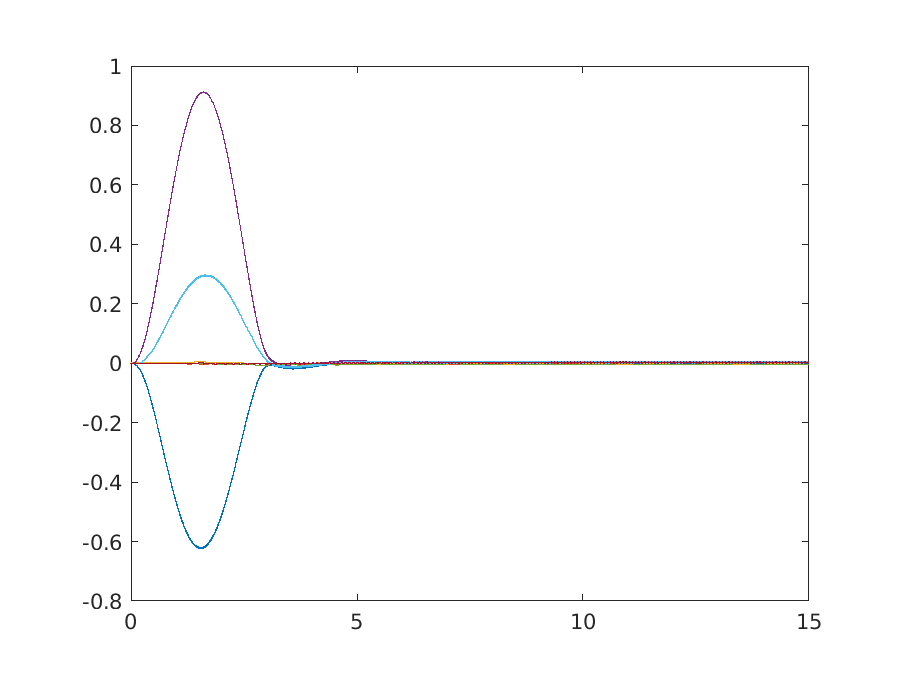
\includegraphics[width=0.8\textwidth]{Figures/est_qp.eps}
      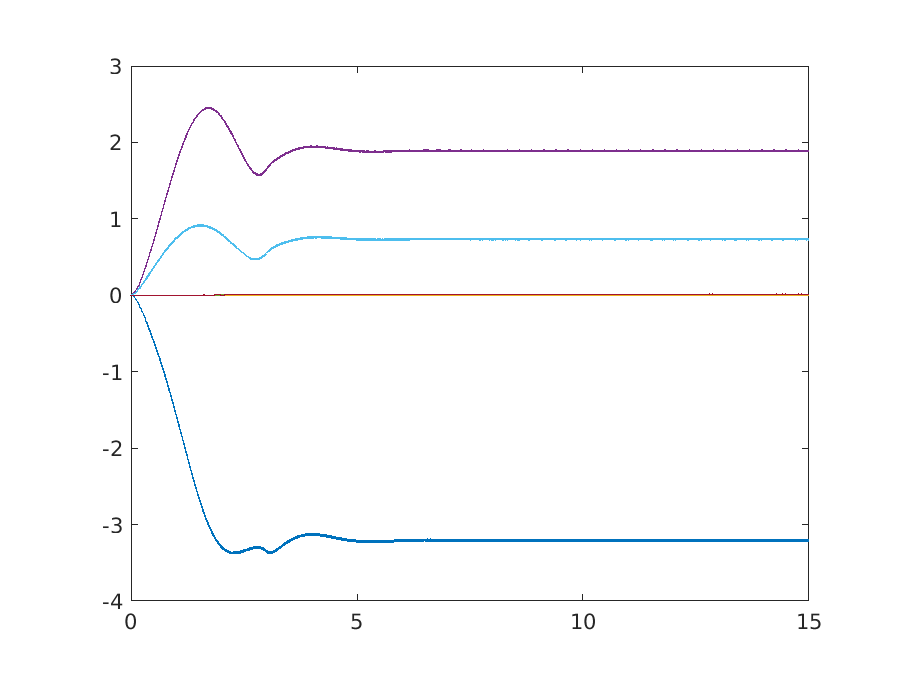
\includegraphics[width=0.8\textwidth]{Figures/controls.eps}
    \end{column}
    \begin{column}{0.5\textwidth}
      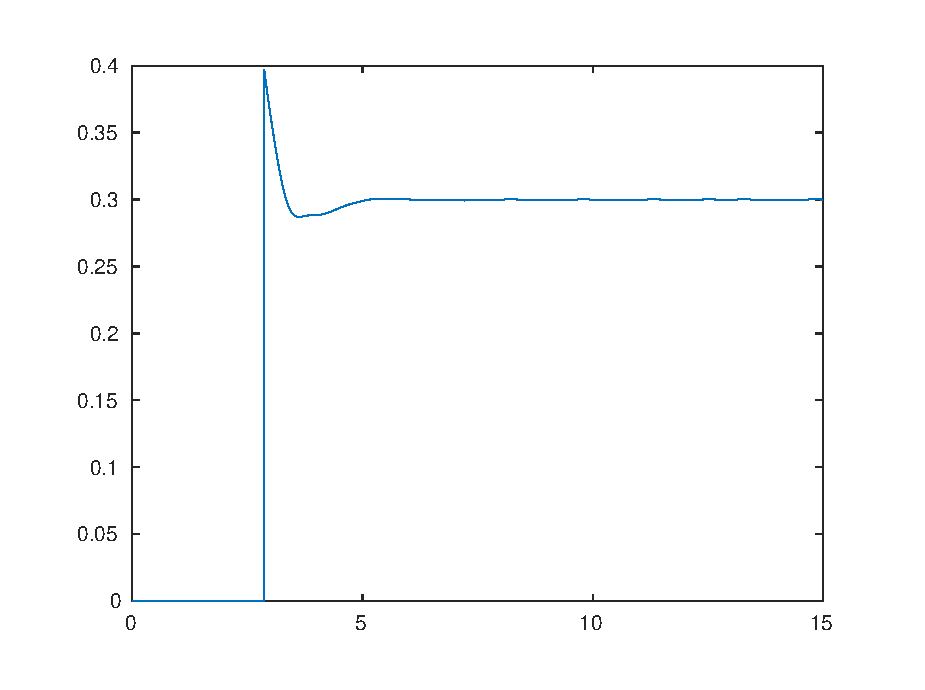
\includegraphics[width=0.8\textwidth]{Figures/est_mass.eps}
      %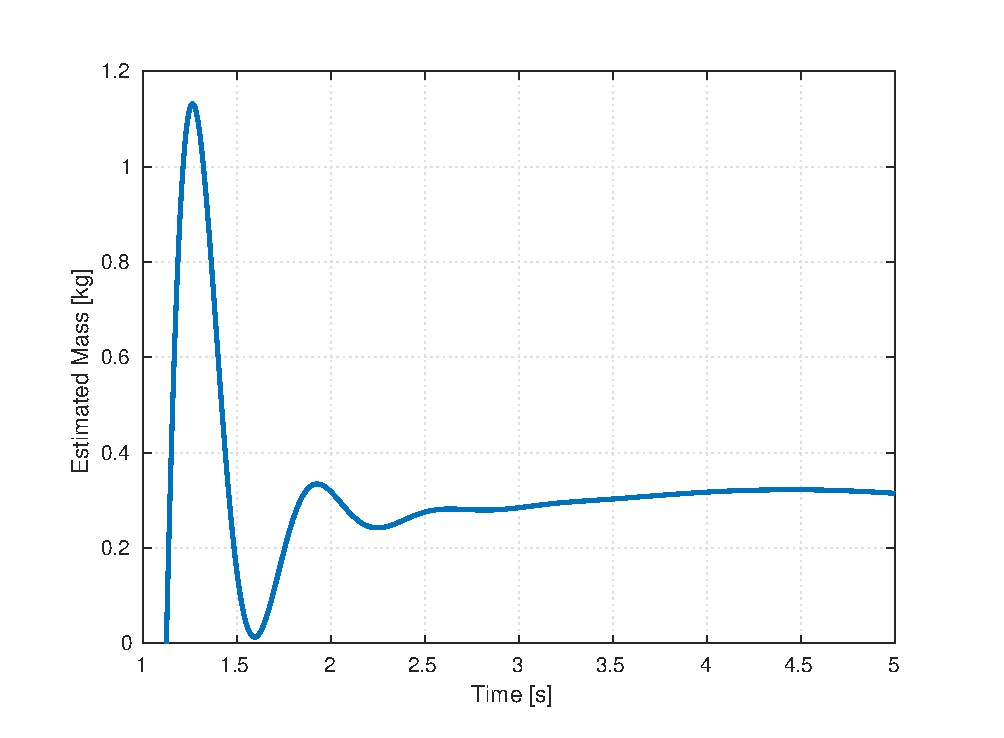
\includegraphics[width=0.8\textwidth]{Figures/estimated_mass_zoom.eps}
    \end{column}
  \end{columns}
\end{frame}

\begin{frame}\frametitle{Next Steps}
\begin{itemize}
\item Estimate the model parameters (still need to determine if doing it by SM techniques or some other approach)
\item Test with the \textit{smooth} version of sliding modes to avoid greater chattering when sampling time increases.
\item Characterize estimation errors due to uncertainties in model parameters.
\item Further exploration on the model structure to allow mass estimation with movements outside the XY plane and before steady state.
\end{itemize}  
\end{frame}
\end{document} 
